%------------------------------------------------------------------------------
% Preamble
%------------------------------------------------------------------------------
\documentclass[]{proposalnsf}

\usepackage{wrapfig,amsmath,amssymb,natbib,mathrsfs,mathtools}
\usepackage{hyperref}
\usepackage{mathrsfs}
%\usepackage{url}
\usepackage{graphicx}
\graphicspath{{./Figures/}} % Tell LaTeX where it should look for your figures.

% For groups of figure folders you can do this...
% \graphicspath{{subdir1/}{subdir2/}{subdir3/}...{subdirn/}} 

% NSF proposal generation template style file.
% Based on latex stylefiles  written by Stefan Llewellyn Smith and
% Sarah Gille, with contributions from other collaborators.
\DeclareFontFamily{OT1}{psyr}{}
\DeclareFontShape{OT1}{psyr}{m}{n}{<-> psyr}{}
\def\times{{\fontfamily{psyr}\selectfont\char180}}

\renewcommand{\refname}{\centerline{References cited}}

% this handles hanging indents for publications
\def\rrr#1\\{\par
\medskip\hbox{\vbox{\parindent=2em\hsize=6.12in
\hangindent=4em\hangafter=1#1}}}

\def\baselinestretch{1}

%------------------------------------------------------------------------------
% End preamble
%------------------------------------------------------------------------------

\begin{document}

%------------------------------------------------------------------------------
\begin{titlepage}

	\centering
	{\scshape\large Geoph 677 final project\par}
	\vspace{3cm}
	{\huge\bfseries Supercycles and Great Earthquakes\par}
	\vspace{2cm}
	{\Large\itshape Rebekah Lee\par}
	\vspace{.5cm}
	{\large \today\par}
	% \vfill
	% supervised by\par
	% Dr.~Mark \textsc{Brown}

	\vfill
	% {\scshape\Large Geoph 677 final project\par}
	{\scshape\Large Boise State University \par}
% Bottom of the page
	
\end{titlepage}

%------------------------------------------------------------------------------
% \title{Supercycles}
% \author{Rebekah Lee}
% \maketitle

\clearpage
\setcounter{page}{1}

%------------------------------------------------------------------------------
\section*{Abstract}
%------------------------------------------------------------------------------

Great earthquakes such as in Sumatra (2004) and Japan (2011) have highlighted our need to better understand long term behavior of subduction zones and other major fault areas. Paleoseismic data offers much needed data that can, in some cases, be used to construct longer time series. Turbidites in particular record relative shaking in the Cascadia subduction zone. \citet{Goldfinger2013} use turbdidite thickness to model relative energy release and construct a 10k time series that shows neither time nor slip predictability. Their time series shows that the 1700 AD event may be typical of the subduction zone and that much larger events have occurred in the past. \citet{Herrendorfer2015} use numerical modeling to investigate the link between subduction zone width and the type of seismic cycle. They find that larger than average width produces supercycles with smaller ruptures transferring stress toward the center of the seismogenic zone. These smaller events prepare the way for a crack-like event that ruptures the entire zone when the overall strength excess is critically low.


%------------------------------------------------------------------------------
% Main body begins here
%------------------------------------------------------------------------------
\section{Introduction}
\begin{figure}
	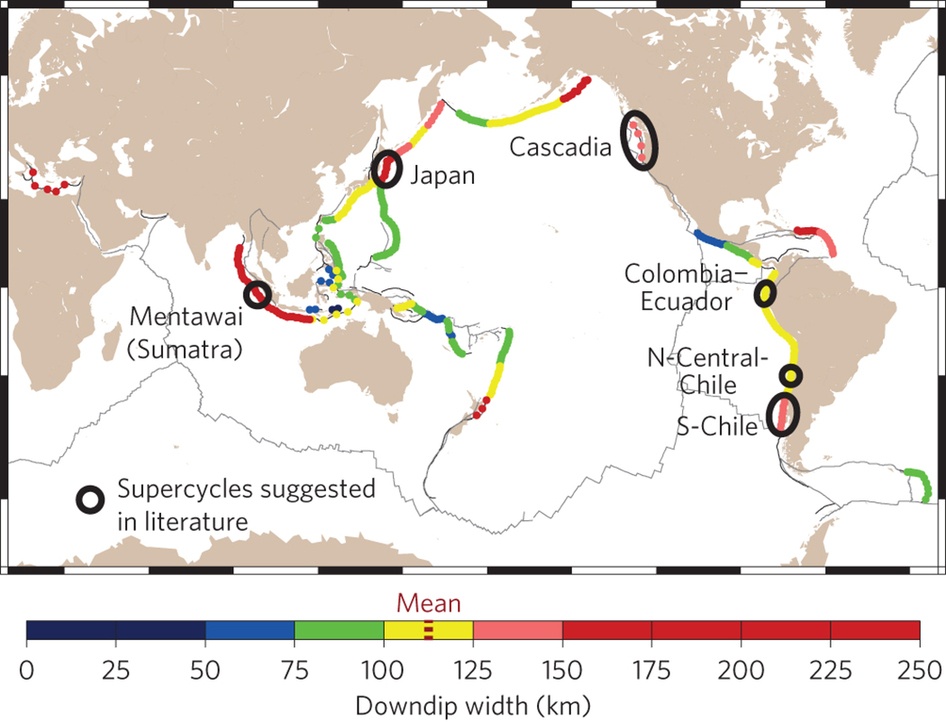
\includegraphics[width=1\linewidth]{Figures/Herrendorfer/ngeo2427-f1.jpeg}
	% 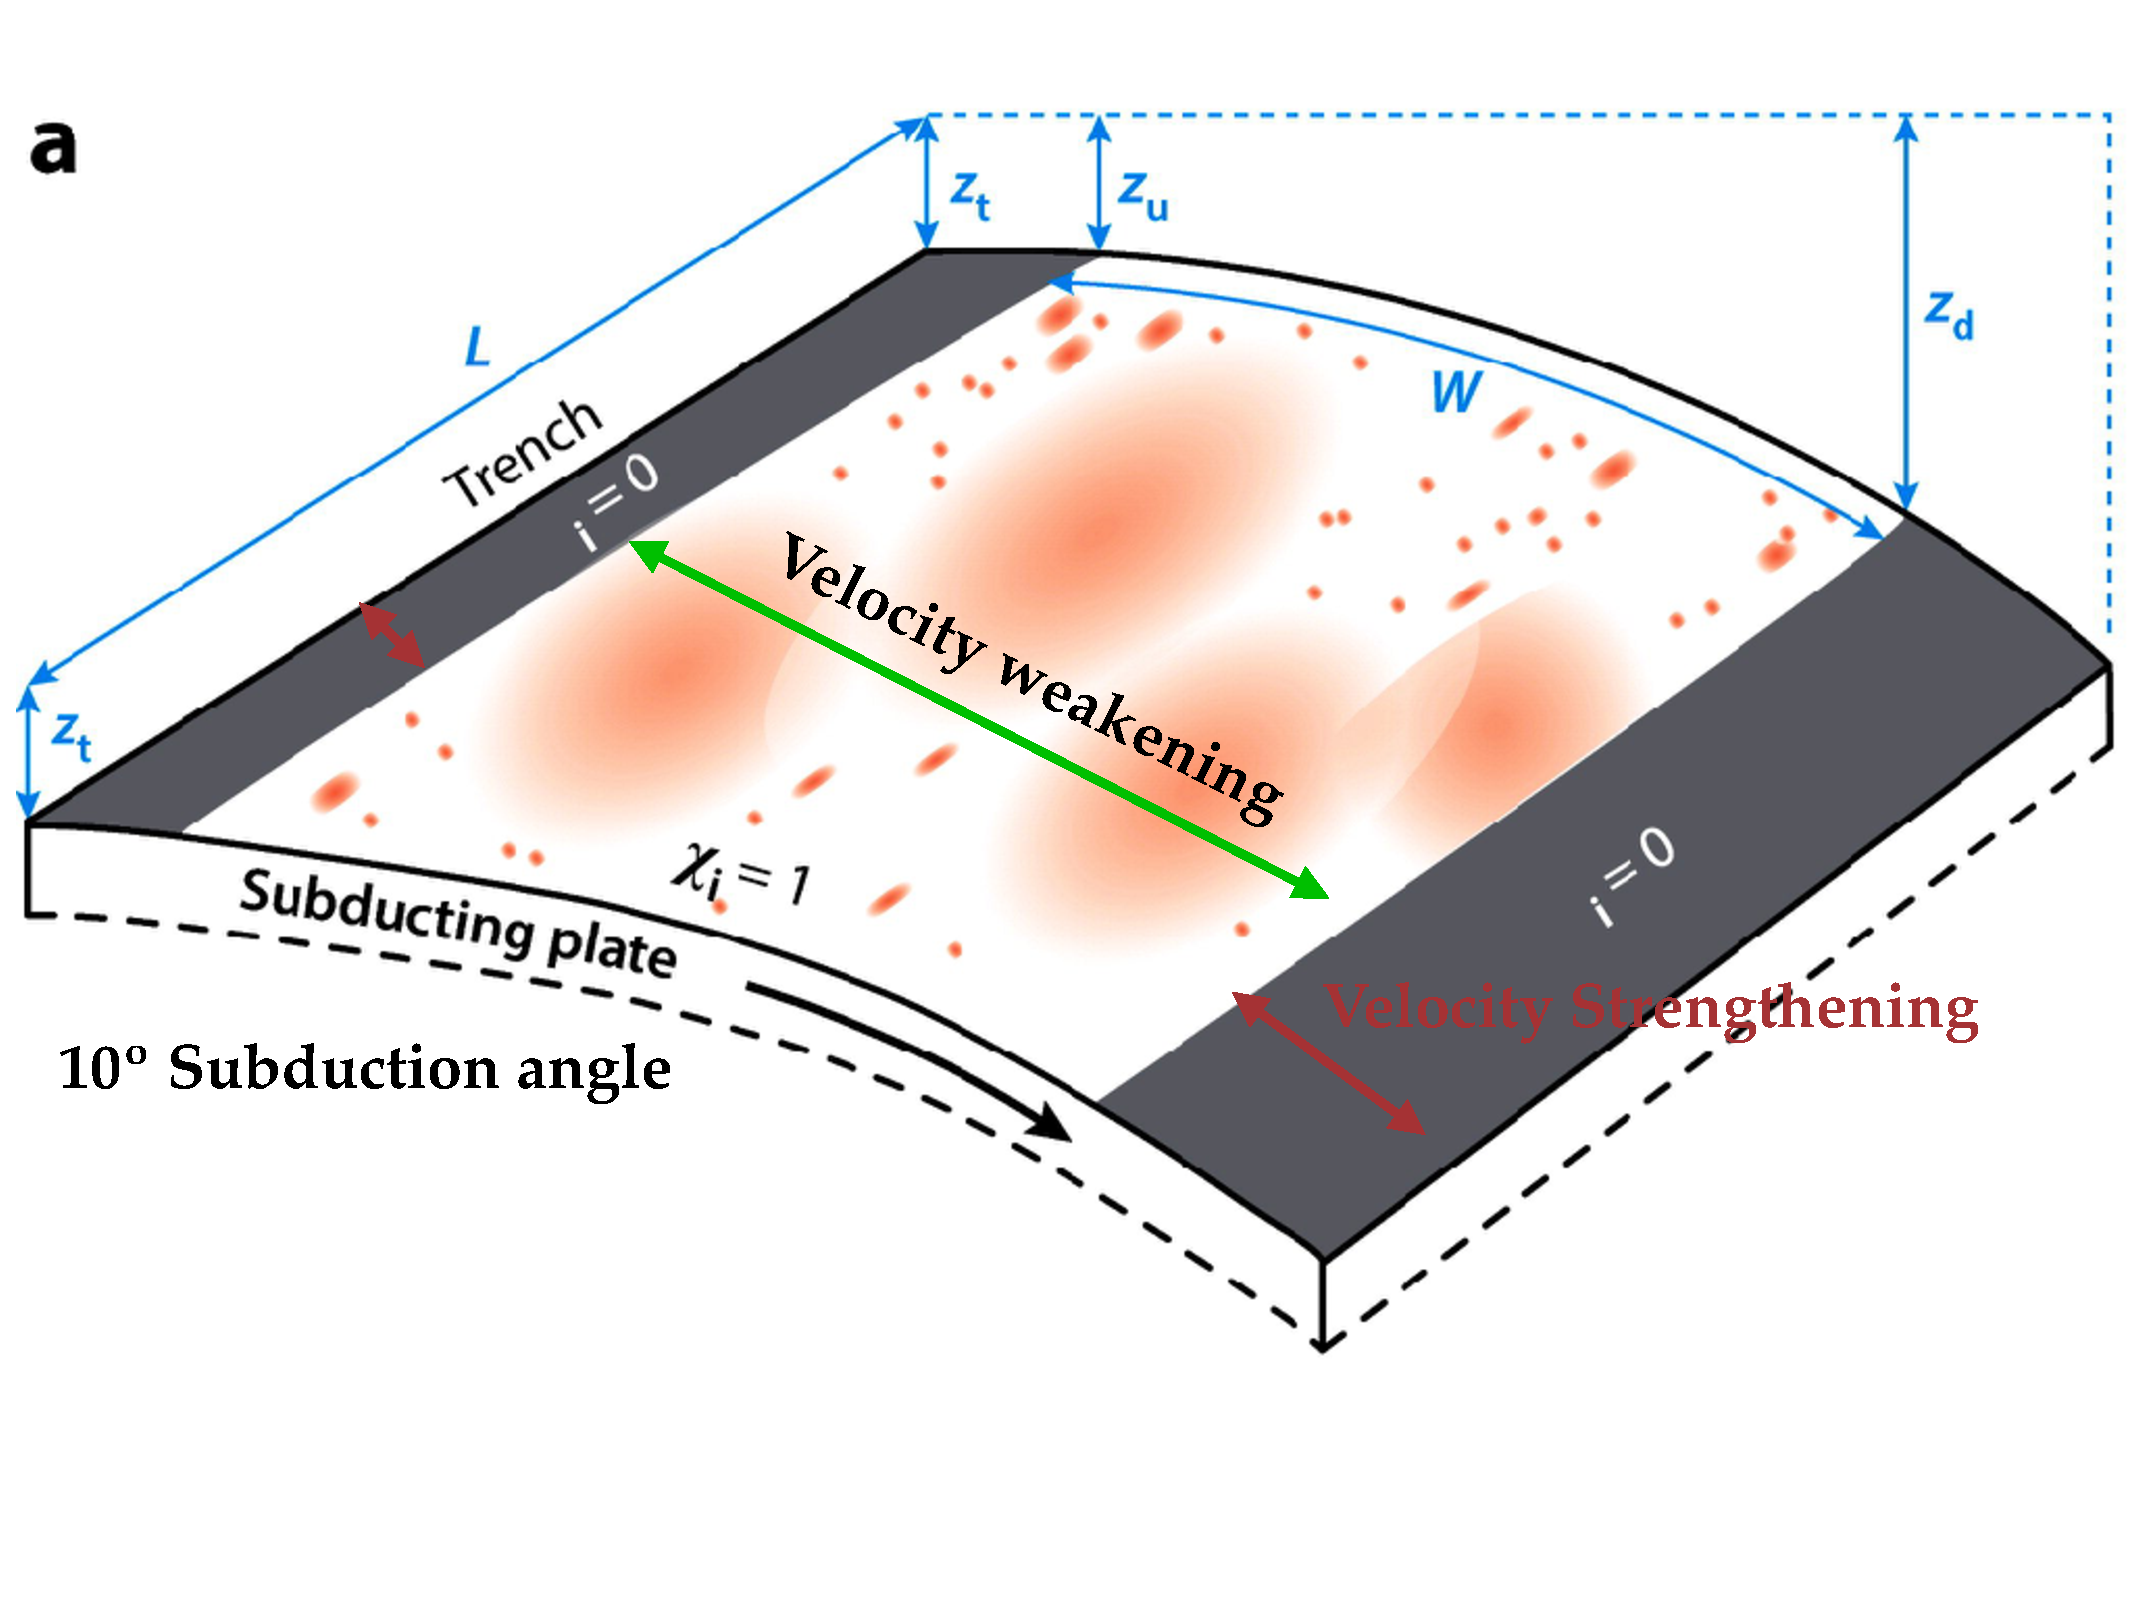
\includegraphics[width=.47\linewidth]{Figures/model.pdf}
	\caption{ Average subduction zone widths and suggested supercycle subduction zones. From \citet{Herrendorfer2015}}
	\label{fig:supercycles}
\end{figure}
Simple relationships to predict the largest magnitude earthquake of a fault zone often fail to predict where, or how large, the next earthquake will be. In 2016, a $M_w$ 7.8 earthquake in Pedernales, Ecuador ruptured an area that overlapped a similar earthquake in 1942. The magnitude of the 2016 event exceeded predicted magnitude from accumulated stress from 1942 \citep{Nocquet2016}. Other infamous examples of larger than expected events include the 2004 Sumatra and 2011 Tohoku, Japan earthquakes. Both were close to $M_w 9$ and generated devastating tsunamis in regions previously thought to have maximum expected earthquake magnitudes of $\sim 8.4$. Each of these events demonstrates the need for further investigation of subduction zones to understand the long term behavior of these fault systems. 

Since the 2004 Sumatra event, there has been more investigation into the cycles controlling subduction zones. In ordinary seismic cycles, large ($ M_w >$ 7) and great ($M_w >$ 8.5) earthquakes release elastic strain accumulated during the previous interseismic period at highly locked asperities, resetting the slip and moment deficit \citep{Nocquet2016}. This implies a local reduction in seismic hazard. The next segment to rupture would be the one with no recent seismic activity. This intuitive relationship is referred to as the seismic gap theory. 

The seismic gap theory does not work well in reality. The same segment can rupture sooner and with larger magnitude than expected based on convergent rate \citep{Nocquet2016}. This suggests that some earthquakes can borrow energy from previous seismic cycles. When this occurs, a cluster of smaller earthquakes can lead to a superevent, greater than magnitude 8.5. This cluster of events is referred to as a supercycle. 

Literature related to supercycles has identified several potential segments of subduction zones thought capable of producing supercycles \citep{Goldfinger2013, Herrendorfer2015, Nocquet2016}. These areas have been identified through paleoseismic and geological data due to the short time period of historical and seismological data. Figure ({\bf \ref{fig:supercycles}}) shows some of these potential supercycle subduction zones. \citet{Herrendorfer2015} observe that all areas of suggested supercycles have larger than average downdip width. They hypothesize that the larger than average width of the seismogenic zone is a controlling factor on producing ordinary or super seismic cycles. 

In the following sections, I will review case studies from \citet{Goldfinger2013}, paying particular attention to the Cascadia subduction zone, and then describe the numerical modeling from \citet{Herrendorfer2015}. The case studies demonstrate how we might extract time series of events on longer time scales. Numerical modeling can also aid in investigating controlling parameters and their relative importance in describing cyclic behavior of subduction zones.

%------------------------------------------------

\section{Methods}

\subsection{Case Studies}

Paleoseismic data can be used where historical and instrumental data are insufficient. Historical and instrumental records have too short durations to characterize long term behavior of a fault system. \citet{Goldfinger2013} give an overview of some of the paleoseismic data and methods available in three case studies: Japan,the Himalayan front, and the Cascadias. I will review the results from Japan and the Himalayan front in the next section.

 The Cascadia case study, in particular, demonstrates how paleoseismic data can be used to construct a longer time series of past events. The authors use turbidites to construct a 10k year time series before present. Turbidites are deposits from slope failure along the continental margin at river deltas. These failures can be caused by excessive sediment load or by shaking from earthquakes. \citet{Goldfinger2013} correlate events from turbidite cores across different depositional environments. This suggests that these deposits were created by shaking from earthquakes. They model coseismic energy release as proportional to mass of turbidite triggered in shaking and assume that between events strain energy accumulates in proportion to the plate convergence rate. They also assume coupling coeffiecient of one and a zero net energy gain over the time series. I show their resulting time series in the next section. 

\subsection{Numerical Modeling}
% \begin{figure}
% \centering
% 	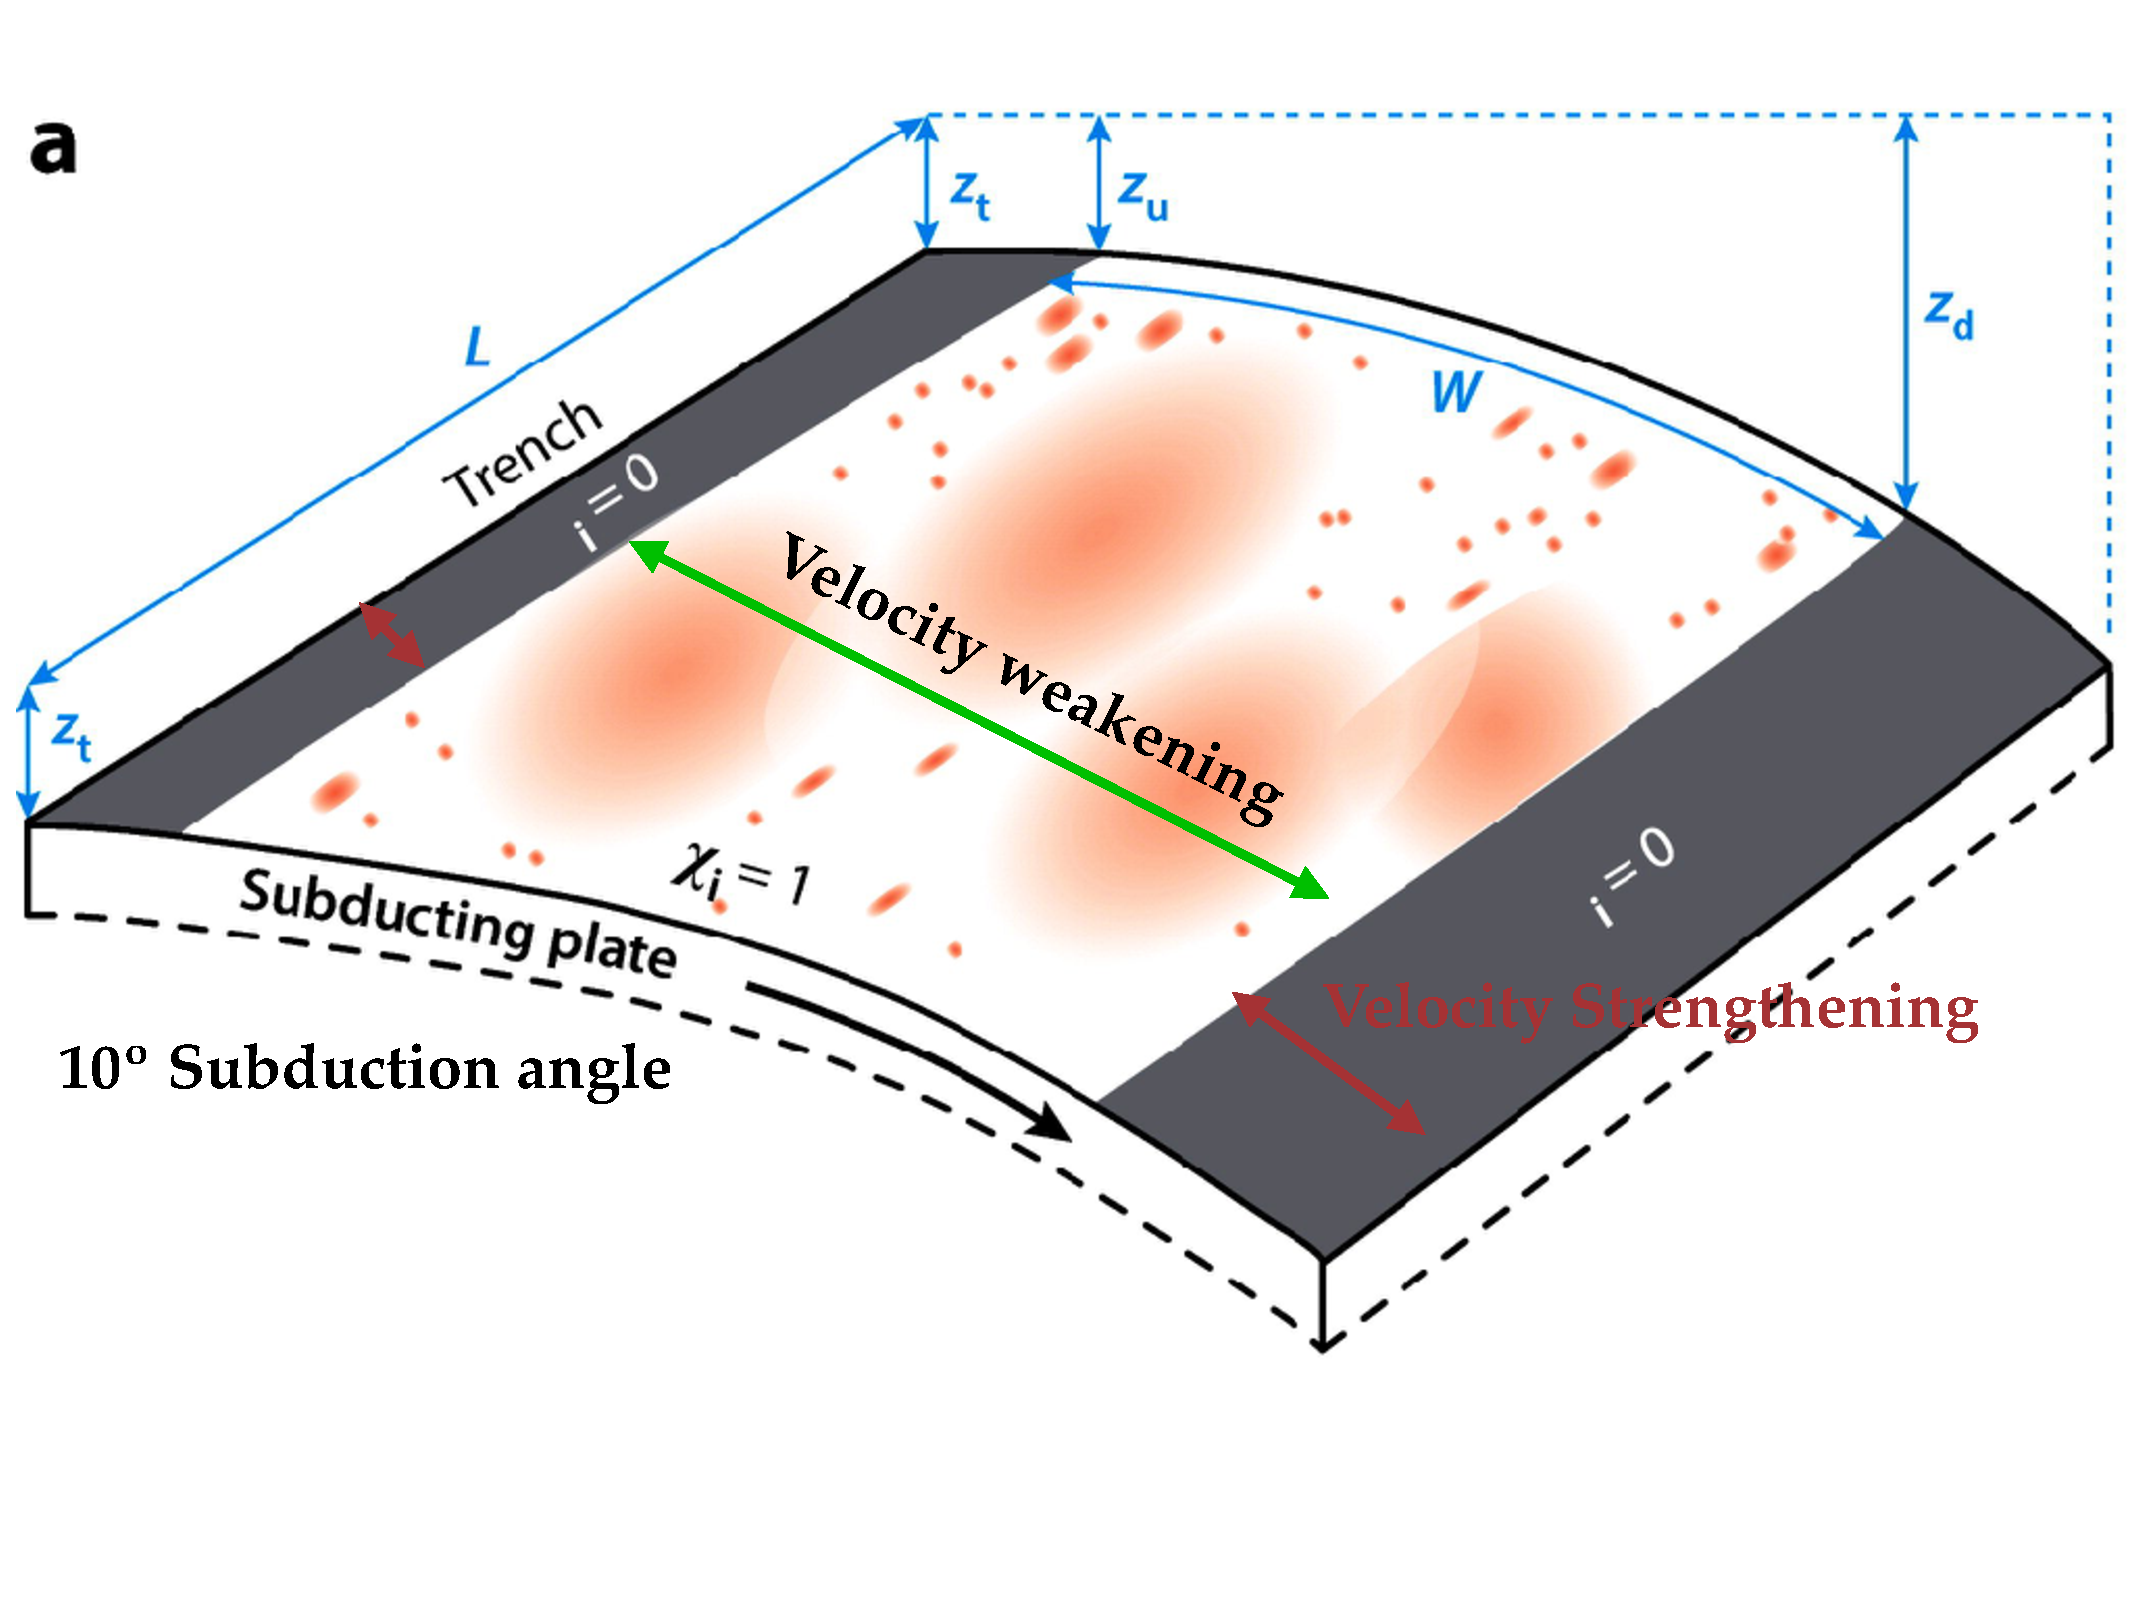
\includegraphics[width=.6\linewidth]{Figures/model.pdf}
% 	\caption{Illustration of model used by \citet{Herrendorfer2015}. }
% \end{figure}

\citet{Herrendorfer2015} test the link between the width of the seismogenic zone and the type of earthquake cycle using a two-dimensional numerical model of a simplified and scaled subduction zone. In their model, a rigid plate subducts beneath a visco-elastic wedge at an angle of $10^\circ$. The seismogenic zone has velocity weakening properties, whereas the aseismic zone has velocity strengthening properties. They use conservative finite differences to solve for conservation of mass (eq. \ref{eqn:mass}) and momentum (eq. \ref{eqn:momentum}) under the assumption of incompressibility ($\nabla \cdot \vec{v}$):
\begin{equation}
	\frac{\partial v_x}{\partial x} + \frac{\partial v_y}{\partial y} = 0,
	\label{eqn:mass}
\end{equation}
\begin{eqnarray}
\frac{\partial \sigma'_{xx}}{\partial x} + \frac{\sigma'_{yy}}{\partial y} - \frac{\partial P}{\partial x} = \rho\frac{Dv_x}{Dt} \nonumber 
\end{eqnarray}
%
\begin{equation}
	\frac{\partial \sigma'_{yx}}{\partial x} + \frac{\sigma'_{yy}}{\partial y} - \frac{\partial P}{\partial y} = \rho\frac{Dv_y}{Dt} - \rho g
	\label{eqn:momentum}
\end{equation}
%
where $v_x$ and $v_y$ are horizontal and vertical velocities, $\sigma'$ is the stress tensor, P is pressure, g is the gravitaional constant, and $\rho$ is density. 

A constitutive relationship connects the deviatoric stresses ($\sigma'_{ij}$) and strain rates ($\dot{\epsilon}'_{ij}$):
%
\begin{equation}
  \dot\epsilon'_{ij} = \frac{1}{2G} \frac{D\sigma'_{ij}}{Dt} + \frac{1}{2\eta}\sigma'_{ij}
  \begin{cases}
        0 & \text{for $\sigma'_{II} < \sigma_{yield}$} \\
        \chi\frac{\partial\sigma'_{II}}{\partial\sigma_{ij}} & \text{for $\sigma'_{II} = \sigma_{yield}$}, 
  \end{cases}
\end{equation}
where G is shear modulus, $\eta$ is effective viscosity, $\sigma'_{II} = \sqrt{\sigma'^2_{xx} + \sigma'^2_{xy}}$ is the plastic flow potential, and $\chi$ is a plastic multiplier connecting plastic strain rates and stresses.

Flow becomes plastic when the plastic flow potential, $\sigma'_{II}$ reaches the local pressure-dependent yield strength, $\sigma_{yield}$:

\begin{equation}
	 	\sigma'_{II} = \sigma_{yield} = C + \mu_{eff} \cdot P, 
 \end{equation} 
where C is cohesion and $\mu_{eff}$ is the effective friction coefficient. $\mu_{eff}$ is strongly rate dependent as it depends on the visco-plastic slip velocity, $V_{vp}$:
\begin{equation}
 	\mu_{eff} = \mu_s(1-\gamma) + \mu_s\frac{\gamma}{1 + \frac{V_{vp}}{V_c}},
 \end{equation} 
 where  $\gamma$ is amount of weakening ($1 - \frac{\mu_s}{\mu_d}$), $\mu_s$ and $\mu_d$ are static and dynamic coefficients, respectively, and $V_c$ is characteristic slip velocity. 

% During plastic deformation elastic strain is zero and the second invariant of deviatoric stresses must be constant. The total strain rate therefore is the sum of the viscous and plastic strain rates, so that the plastic strain is $\dot{\epsilon}'_{II} - \dot{\epsilon}'^{(viscous)}_{II}$ (where $\dot{\epsilon}'_{II} = \sqrt{\dot{\epsilon}'^2_{xx} + \dot{\epsilon}'^2_{xy}}$ ) and the visco-plastic viscosity is:
% \begin{equation}
%  	\eta_{vp} = \eta\frac{\sigma'_{II}}{\eta\chi + \sigma'_{II}},
%  \end{equation} 
% with 
% \begin{equation}
% 	\chi = 2(\dot{\epsilon}'_{II} - \dot{\epsilon}'^{(viscous)}_{II}) = 2(\dot{\epsilon}'_{II} - \frac{1}{2\eta}\sigma'_{II})
% \end{equation}
After solving for the horizontal velocity, \citet{Herrendorfer2015} analyze their models using a set of functions at each time time step and averaging over the width of the seismogenic zone. Among these functions are the cumulative sum of the displacements, D, and strength excess, SE. The displacement tracks the accumulated elastic strain through time:
%
\begin{equation}
D(t) = \frac{1}{W} \sum_{j=1}^t \sum_{x=d}^u V(x,j)\cdot \Delta t \cdot \Delta x,	
\end{equation}
where $u$ is the updip limit and $d$ is the downdip limit. The strength excess represents the stress and strength state of the seismogenic zone:
\begin{equation}
	SE(t) = \frac{1}{W}\sum_{x=d}^u (\sigma_{yield}(x,t) - \sigma '_{II}(x,t)) \cdot \Delta x.
\end{equation}
 A low strength excess indicates that the zone is close to a critical state at which ruptures of the entire zone are likely to occur.

%-----------------------------------------------------------------------------------------------------------
%									Data and Results
%-----------------------------------------------------------------------------------------------------------
\section{Data and Results}

\subsection{Case Studies from Paleoseismic Data}

\subsubsection{Japan Trench and Himalayan Front}

For the Japan case study, \citet{Goldfinger2013} review the tsunami record. In the Sendai area of Japan, there is record of an event in 869 as well as two predecessors that each produced a tsunami reaching 3-4 km inland, similar to the 2011 earthquake. These large tsunamis support the existence of periodic outsized earthquakes (greater than $M_w$ 9) with recurrence intervals between 800-1200 years. 

Along the Himalayan front, paleoseismic evidence shows earthquakes that produced surface displacement of up to 26 meters.  Four modern earthquakes between 1897 and 1950 reached the maximum considered earthquake with magnitudes between 7.8 and 8.4. However, none of the modern events have produced surface rupture. This suggests that the front is capable of producing even more damaging earthquakes. The Japan and Himalayan cases studies both suggest that the maximum magnitude a fault system is capable of producing may be unknown. 

\begin{figure}
% \hspace{-1cm}
	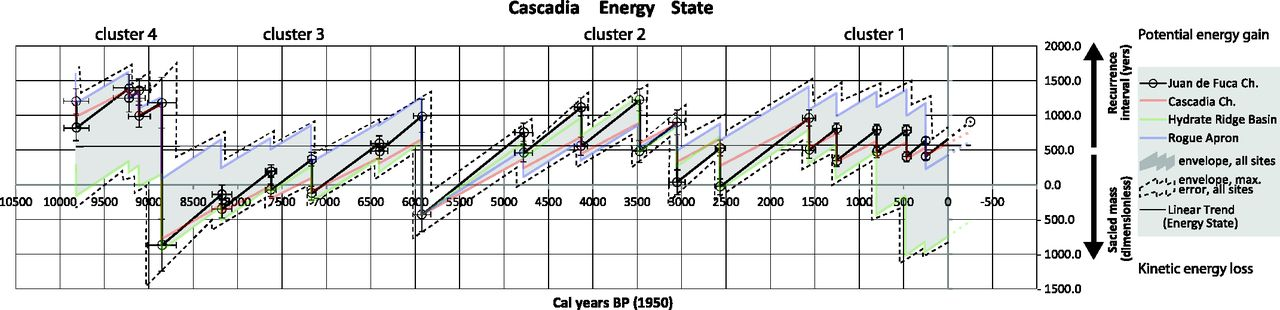
\includegraphics[width=1\linewidth]{./Figures/Goldfinger/F4large.jpg}
	\caption{Energy Cycle of the Cascadia subduction zone. Energy gain is proportional to recurrence interval and energy loss to mass of turbidite samples. Vertical axis shows relative energy gain/loss and is dimensionless. From \citet{Goldfinger2013}}
	\label{fig:energyCycle}
\end{figure}

\subsubsection{Cascadian Subduction Zone}

 \citet{Goldfinger2013} identify four seismic clusters in their time series of the Cascadian subduction zone. Figure {\bf \ref{fig:energyCycle}} shows the the time series modeling the energy state using the turbidite mass and thickeness. Beginning from 10 thousand years before present (1950), cluster four shows an even energy state before falling to a low after a large event. Cluster three climbs steadily until falling to a similar low. During this period there are several seismic cycles with relatively low stress drops that do not relieve all of the accumulated strain. A total stress drop finally happens at the end of the cluster with an event much larger than the others within the same cluster. Cluster two differs from the previous in that it does not culminate in an over-sized event. Rather, it climbs and then falls over several seismic cycles until it reaches a low energy value about 2500 years BP. The end of the cluster marks a long gap of about 1,000 years of constant increase in energy. Cluster one then slowly decreases the energy state until the A.D. 1700 $M_w$ ~9.0 earthquake. From the time series, it appears that the 1700 event is not atypical, suggesting that the region may be capable of producing even greater magnitude events. 

The four clusters modeled by \citet{Goldfinger2013} demonstrate that some events in this subduction zone release energy from previous cycles. This subduction zone is neither slip nor time predictable. Energy release is not tied to recurrence intervals as some events can release energy accumulated from previous seismic cycles. High energy states results in one very large event, (as in the case of cluster four), or a series of smaller events (as in cluster two). Low energy state results in a long gap in seismicity (cluster two) or a series of small earthquakes with net energy gain over several cycles (cluster three). 

The Cascadia case study indicates that we may not have seen the largest earthquakes this area can produce. Other subduction zone could also be capable of producing supercycles. Zones of supercycles represent areas with a potentially devastating culminating event. Given this potential, it is import to investigate what may control supercycle behavior.

\begin{figure}
	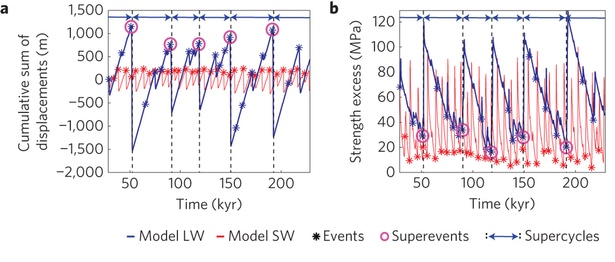
\includegraphics[width=1\linewidth]{Figures/Herrendorfer/ngeo2427-f2_edit.jpg}
	\caption{Comparison of characteristics of long (LW) and small (SW) downdip width subduction zone models. Earthquakes indicated by astericks and superevents are circled. Subfigures show cumulative sum over time ({\bf a}) and excess strength ({\bf b}). From \citet{Herrendorfer2015}.}
	\label{fig:SZOwidth}
\end{figure}
\begin{figure}
	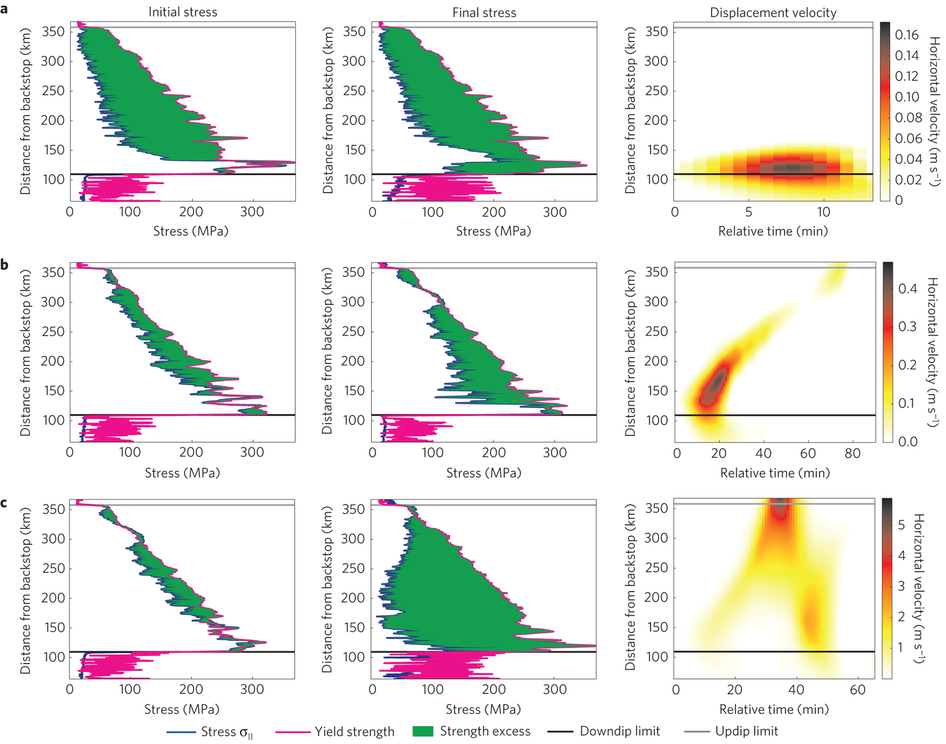
\includegraphics[width=1\linewidth]{Figures/Herrendorfer/ngeo2427-f3.jpeg}
	\caption{Rupture styles in LW reference model. Subcritical rupture (a), pulse-like rupture (b), and crack-like rupture (c). Left column shows initial state just before rupture while middle column shows the final state. The excess strength is shaded green and is the difference between the stress and yield strength. The right column shows the spatiotemporal evolution of the horizontal velocity during rupture. From \citet{Herrendorfer2015}}
	\label{fig:ruptureStyle}
\end{figure}

\subsection{Controls to type of Seismic Cycle}
\citet{Herrendorfer2015} test the link between seismogenic zone width and the type of seismic cycle. Figure {\bf \ref{fig:SZOwidth} (a-b)} show results from two end models. The large width (LW) seismogenic zone has a width of 248 Km and is plotted in blue. The small width (SW) model has a width of 102 Km and is plotted in red. 

Both models show that events are triggered at low excess stress (Figure {\bf \ref{fig:SZOwidth}b}). The LW model events, however, have much greater magnitudes (represented by displacement in figure {\bf \ref{fig:SZOwidth}a}) at similar low stresses to the SW model. Large width zones are characterized by supercycles that partially release stress but overall excess strength continues to decrease to a low level, at which point a superevent occurs. 

The authors define three different types of events in the LW model. Column three of figure {\bf \ref{fig:ruptureStyle}} shows plots of the horizontal velocity through time and distance from backstop for each of the rupture types. The first type of ruptures they call subcritical ({\bf \ref{fig:ruptureStyle}a}) and are events that fail to propagate a long distance out of their nucleation region but last for the duration of the rupture. The second, pulse-like ({\bf \ref{fig:ruptureStyle}b}), ruptures propagate further than subcritical ruptures but have a local duration of coseismic displacements that is short compared to the total rupture duration. Finally, in a crack-like rupture ({\bf \ref{fig:ruptureStyle}c}) most of the rupture area continues to slip until the end of the rupture. 

Figure {\bf \ref{fig:ruptureStyle}} shows strength excess (shaded green) before and after each of the event types in the first two columns. Subcritical events ({\bf \ref{fig:ruptureStyle}a}) nucleate close to the downdip limit of the seismogenic zone and transfers stress close to the stopping location (about 125 km from backstop). Pulse-like ruptures ({\bf \ref{fig:ruptureStyle}b}) nucleate from the downdip limit for short duration and transfer stress updip (about 300 km from backstop). These combine to shift the strain towards the center of the seismogenic zone that eventually results in the crack-like event ({\bf \ref{fig:ruptureStyle}c}) that ruptures the entire zone. 

The width of the seismogenic zone controls the overall strength excess. Small width zones have lower overall strength excess and are characterized by crack-like events. The average strength excess is increased by increased width and leads to transition from crack-like ruptures of the entire zone to subcritical and pulse-like ruptures that prepare the entire zone for the culminating crack-like rupture. 

%------------------------------------------------

\section{Conclusion}
Our short instrumental and historical records are unable to characterize the behavior of subduction zones due to their complex nature and long overall recurrance intervals. Examining the geologic record can give us a good indication of whether or not a subduction zone has produced over-sized events in the past. These records include paleoseimic evidence, tsunami observations, and turbidite deposits. Recent great earthquake events demonstrate that there are exceptions to simple relationships such as convergent rate and plate age to predict the size of earthquakes in subduction zones. One reason for this is that supercycles can use energy from previous seismic cycles. The 2004 Sumatra and 2011 Japan events demonstrate the need for scientists and engineers to reexamine what the maximum expected earthquake could be for a given subduction zone. 

When paleoseismic data is not available, modeling can offer important insights into parameters that might push a fault zone into a supercyle. \citet{Herrendorfer2015} found that larger width of the seismogenic zone can control whether a zone is capable of supercycles. Future modeling could also investigate the along strike length of the subduction zone and the link with supercycles. \citet{Herrendorfer2015} also acknowldege that multiple segments can rupture to produce oversized events. Supercycles are complicated and much more investigation is needed in order to better understand the physics of what produces supercycles and great earthquakes.  





%------------------------------------------------------------------------------
% References Cited 
%------------------------------------------------------------------------------
% See the Grant Proposal Guide for format.
% Reference information is required. Each reference must include the
% names of all authors (in the same sequence in which they appear in
% the publication), the article and journal title, book title, volume
% number, page numbers, and year of publication. If the document is
% available electronically, the Website address also should be
% identified. Proposers must be especially careful to follow
% accepted scholarly practices in providing citations for source
% materials relied upon when preparing any section of the
% proposal. While there is no established page limitation for the
% references, this section must include bibliographic citations only
% and must not be used to provide parenthetical information outside of
% the 15-page project description.

\newpage
% \setcounter{page}{1}

\bibliography{sources}
\bibliographystyle{agufull08}

\end{document}
